\subsubsection{Implementation de l'Univers}
Nous avons choisi de représenter l'univers de jeu de la manière suivante:
\begin{itemize}
\item \textbf{Un univers} est constitué d'un ensemble de monde.Il est caractérisé par un nom, mais aussi par sont ensemble de mondes.
\item \textbf{Un monde} est présent dans un Univers et contient lui-meme plusieurs zones. Un monde est caractérisé par un numéro qui lui est propre, par son nom, mais aussi par un ensemble de zones qui le compose. 
\item \textbf{Une Zone} est présente dans un seul et unique monde et celle-ci contient plusieurs questions. Une zone se caractérise par son numéro unique, son som mais aussi un ensemble de questions qui sont liées à cette zone.
\item \textbf{Une question} est relative à une et une seul zone. Celle-ci est caractérisée par: \begin{itemize}
					\item Un nom qui lui est propre.
					\item L'intitulé de cette question qui sera affichée au joueur.
					\item Un ensemble de propositions relatives à cette question.
					\item Le nombre de propositions que cette question possède.
				  \end{itemize} 
\item \textbf{Une proposition} est quand à elle est relative à une et une seule question.
Elle se caractérise par:\begin{itemize}
							\item Le libellé de la proposition qui seras affiché au 									  joueur.
							\item Le nombre de point que rapporte la proposition si 		   							  celle-ci est choisie.
							\item Le nombre de point minimum pour que la proposition 		   							  s'affiche au joueur.
							\item Le nombre de point maximum à partir duquel la 		                                  proposition ne s'affiche plus au joueur.
							\item Un éventuel lien vers un monde si cette proposition 									  renvoit vers un autre monde. 
							\item Une liste de liens vers différentes zones vers 			   							  lequels peut renvoyer la proposition.
							\item La reponse à la proposition qui serat affichée 	  									  lorsque l'utilisateur selectionneras la proposition.   
					    \end{itemize}
					    
\end{itemize}
Ci dessous, un schéma récapitulatif de l'organisation de l'Univers de Jeu.
\begin{figure}[h]
	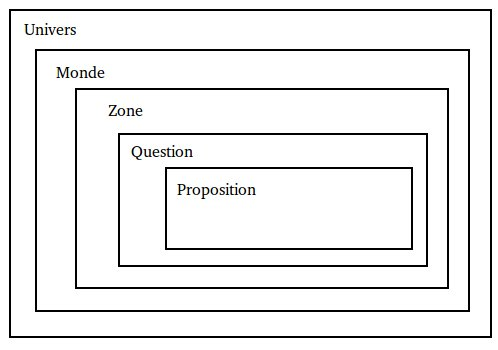
\includegraphics[scale=0.8]{figures/schema-univers.jpg}
	\caption{Schema récapitulatif de l'Organisation de l'Univers de jeu}
\end{figure}